%
% 修士学位請求論文(副・正)テンプレート
% MasterThesisSample.tex
% By KASHINA, Yuki (EM-14003)
%
\documentclass{MasterThesis}
%\documentclass[fleqn]{MasterThesis} %数式を左寄せ


%%%%%%%%%%%%%%%%%%%%%%%%%%%%%%%%%%%%%%%%%%
% ユーザ任意のパッケージ
%%%%%%%%%%%%%%%%%%%%%%%%%%%%%%%%%%%%%%%%%%
%\usepackage{booktabs}
%\usepackage{multirow}
\usepackage[dvipdfmx]{xcolor}
\usepackage{otf}


%%%%%%%%%%%%%%%%%%%%%%%%%%%%%%%%%%%%%%%%%%
% マクロ
%%%%%%%%%%%%%%%%%%%%%%%%%%%%%%%%%%%%%%%%%%
%<local definition>
\newcommand{\texcmd}[1]{\texttt{\textbackslash{}#1}}

\usepackage{setspace}
\def\commentary#1{\raisebox{\baselineskip}{\parbox{0.8\textwidth}{\begin{spacing}{0.8}#1\end{spacing}}}\vspace{.42\baselineskip}\endgraf}
%</local definition>


%%%%%%%%%%%%%%%%%%%%%%%%%%%%%%%%%%%%%%%%%%
% ルートパス
%%%%%%%%%%%%%%%%%%%%%%%%%%%%%%%%%%%%%%%%%%
\graphicspath{{figure/}}
\tablepath{{table/}}


%%%%%%%%%%%%%%%%%%%%%%%%%%%%%%%%%%%%%%%%%%
% 行間調整
%%%%%%%%%%%%%%%%%%%%%%%%%%%%%%%%%%%%%%%%%%
\renewcommand{\baselinestretch}{1.0}


%%%%%%%%%%%%%%%%%%%%%%%%%%%%%%%%%%%%%%%%%%
% 図表キャプションの接頭辞
%%%%%%%%%%%%%%%%%%%%%%%%%%%%%%%%%%%%%%%%%%
%\renewcommand{\jfigurename}{図}
%\renewcommand{\jtablename}{表}
%\renewcommand{\efigurename}{Fig.~}
%\renewcommand{\etablename}{Table~}


%%%%%%%%%%%%%%%%%%%%%%%%%%%%%%%%%%%%%%%%%%
% フォントサイズ
%%%%%%%%%%%%%%%%%%%%%%%%%%%%%%%%%%%%%%%%%%
%%% 英文タイトル
%\renewcommand{\etitlefontsize}{\fontsize{21pt}{21pt}}
\renewcommand{\etitlefontsize}{\fontsize{14pt}{14pt}}

%%% 本文
%\renewcommand{\mainfontsize}{\fontsize{14pt}{25pt}}
\renewcommand{\mainfontsize}{\fontsize{12pt}{21pt}}

%%% キャプション
%\renewcommand{\captionfontsize}{\fontsize{14pt}{17pt}}
\renewcommand{\captionfontsize}{\fontsize{11pt}{14pt}}


%%%%%%%%%%%%%%%%%%%%%%%%%%%%%%%%%%%%%%%%%%
% 書誌情報
%%%%%%%%%%%%%%%%%%%%%%%%%%%%%%%%%%%%%%%%%%
%%% 和文タイトル
% \newlineで改行,数式やコマンド,クォートは{}でグルーピング
% \jtitle{体験情報に基づくLies-Bias型観光支援システム}{}
\jtitle{ユーザの体験情報を用いた観光支援システム}{}

%%% 英語タイトル・サブタイトル
% \etitle{ユーザの訪問情報を用いた観光支援システム}{}

%%% 所属専攻 //工学研究科は不要
\affiliate{情報学専攻}

%%% 氏名・学籍番号 //\ruby{漢字}{かん|じ}, 性名間に半角空白を挿入
\author{\ruby{潘}{はん}~\ruby{健太}{けん|た}}

%%% 指導教官名・指導教官役職 //姓名間に半角空白を挿入
\supervisor{北山~大輔}{准教授}

%%% 修了年月(西暦) //全角を推奨
\ptdate{2020}{3}

%%% 前文のタイトル
\abstractname{要旨}{Abstract}

%%% 目次の有効化
\toctrue

%%% 図目次の有効化
\loftrue

%%% 表目次の有効化
\lottrue

%%% 索引の有効化
%\makeindex

%%% 研究室内部資料セクション(付録)の有効化
%\domestictrue



%%%%%%%%%%%%%%%%%%%%%%%%%%%%%%%%%%%%%%%%%%
% 書誌情報の設定終了
%%%%%%%%%%%%%%%%%%%%%%%%%%%%%%%%%%%%%%%%%%
\eom



%%%%%%%%%%%%%%%%%%%%%%%%%%%%%%%%%%%%%%%%%%
% 前文(和文)
\jabstract
%%%%%%%%%%%%%%%%%%%%%%%%%%%%%%%%%%%%%%%%%%


%%%%%%%%%%%%%%%%%%%%%%%%%%%%%%%%%%%%%%%%%%
% 本文の開始
%%%%%%%%%%%%%%%%%%%%%%%%%%%%%%%%%%%%%%%%%%
\main



%%%%%%%%%%%%%%%%%%%%%%%%%%%%%%%%%%%%%%%%%%
% はじめに
\chapter{序論}
%%%%%%%%%%%%%%%%%%%%%%%%%%%%%%%%%%%%%%%%%%
一般に,ユーザは観光旅行する前にWeb上の情報やガイドブックを活用して計画を立てることが多くなっている.
その際,目的とする観光スポットに関する概要やアクセスするための方法などの情報を集める.
ガイドブックは,有名な観光スポットや流行りのものに焦点を当て,そのスポットの料金や見どころ,そして食べ物などが掲載されており,その土地に初めて観光で訪れるユーザや,普段から頻繁に観光旅行をしないユーザにとって満足を得られるような内容が書かれている.そのため,ガイドブックは普段から頻繁に観光旅行をするようなユーザや,その観光スポットに対してこだわりの観点を持つユーザの個別の嗜好までは考慮できない.

Web上の情報に関して,観光スポットに関する総合的な情報が掲載された公式サイト,過去にそこを訪れた観光者による旅行記ブログサイト,そして,評価が記載されたレビューサイトなどの様々なサイトがある.
しかしながら,種々のサイトが混在しており,膨大な情報から自分の嗜好に合う観光スポットの情報を得ることは簡単ではない.
目的の情報を収集するためには手動で閲覧し取捨選択しなければならない.
旅行計画を立つために,まず訪問したいエリアを決定する必要がある.
その後,観光スポット検索サイトやガイドブックの観光スポット情報を調べて観光スポットを決定する.
ユーザの意識決定の材料の1つとして,るるぶトラベル\footnote{https://www.rurubu.travel/},Tripadvisor\footnote{https://www.tripadvisor.com/}やじゃらん\footnote{https://www.jalan.net/kankou/}などの観光スポット検索サイトがある.これらのサイトには特定の観光スポットを訪問したことのあるユーザがレビューを投稿し,観光スポットに関する豊富な情報が存在している.
観光スポット検索サイト上で観光スポットに付与される情報の例\footnote{https://www.jalan.net/kankou/130000/?screenId=OUW2201}を図\ref{fig:観光スポット検索サイト上で観光スポットに付与される情報例}に示す.
なお,これらの情報のうちユーザレビュー以外の情報(概要文・タグ・評価点など)はメタデータと呼ばれる.
\begin{figure}[t]
    \centering
    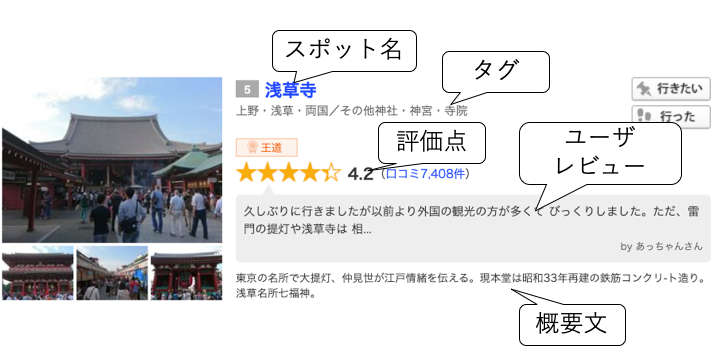
\includegraphics[width=0.9\textwidth]{figure/spot_info.png}
    \caption{レビューサイト上で観光スポットに付与される情報例}
    \label{fig:レビューサイト上で観光スポットに付与される情報例}
\end{figure}

観光スポット検索サイトに掲載された情報を基に,利用者(ユーザ)は自身の嗜好や目的に合致した特徴を持つ対象観光スポットを検索する.
多くの観光スポット検索サイトでは,対象観光スポットに付与されるメタデータを利用した以下のような検索方法が提供されている.

\begin{itemize}
\item ユーザが指定したタグを持つ対象観光スポット
\item 評価点などの数値メタデータに基づく並び替え
\item 入力単語(クエリ)を概要文中に含むオブジェクトの検索
\end{itemize}

しかし,これらのメタデータを用いた検索方法だけでは検索が困難な場合も存在する.
たとえば,対象観光スポットを実際に利用することでユーザが得られる印象・感情・体験などを表す特徴に基づき対象観光スポットを検索したい場合などが該当する.
また,訪問したいエリア内に数多くの観光スポットが存在している.
ユーザは検索エリアに関する事前知識がないため,検索された多数の観光スポットからどの観光スポットのレビューを読むべきか効率的に判断することは困難で,自身のイメージから外れない観光スポットを見つけることは容易ではない.
そこで,本研究では,さまざまな観光スポットを効果的に理解するためには,ユーザが訪問した体験のある観光スポットとを使って未訪問スポットを検索する手法を提案した.
観光支援システムを構築するにあたり課題となる点は2つ説明する.

\begin{enumerate}
\item 観光スポット間の対応付け

ある観光スポットに対応する観光スポットを判定する手法として,レビューやカテゴリが類似したコンテンツであるという観点で判定する方法が一般的である.
観光スポットで用いられる単語に対する従来の特徴量TFIDFは,観光スポット内での重要な単語を判定する際に用いられる.
しかし,従来手法のTFIDFはユーザの観光スポット選択における意図や他スポットへの関心について考慮されていない.
そのため,ある観光スポットが他の観光スポットと比較するとき,その観光スポットの特徴を表すことができない.
そこで,あるスポットに対し,既に訪問した観光スポットと比較した相対的特徴ベクトルを作成し,相対的特徴ベクトル間の類似度に基づいて既訪問スポットと未訪問スポット間の対応付け手法を提案する.第3章で,より具体的な提案手法について述べる.

\item 観光スポットの対応関係を地図上に可視化

地理的情報の可視化を意味的な関係の可視化に取り込む情報の可視化としては,抽出した情報を地図上にマッピングするのが一般的である.また,意味的な関係性の可視化として,グラフモデル上でオブジェクト間のつながりを関連度で表現することが多い.
観光スポット間の意味的な対応関係を可視化するために,未訪問スポットは地図上で実在する座標に固定され,配置の自由があるのは既訪問スポットのみという制約がある.
そこで,ある未訪問スポットに対して,入力した既訪問スポットがどのような関係にあるのか地図上で,一目で把握できるために,既訪問スポットと未訪問スポットの対応関係を可視化する手法を提案する.第4章で,より具体的な提案手法について述べる.
\end{enumerate}

以下に本論文の構成を示す.
ます,2章で本研究のアプローチについて述べる.
ここでは観光支援システムのアルゴリズムと関連研究について述べる.
この観光支援システムのための2つの観点に基づく各手法は3章と4章で述べる.
3章では,ユーザの既訪問スポットの位置付けに基づく未訪問スポットの説明手法について述べる.
4章では,地図上における未訪問スポットの説明向上のための観光スポットの対応付け可視化手法について述べる.
5章では,各手法に対する評価実験結果を踏まえた提案手法全体に対する考察を行う.
6章では,まとめと今後の課題を述べる.


%%%%%%%%%%%%%%%%%%%%%%%%%%%%%%%%%%%%%%%%%%
\chapter{本研究のアプローチ}
%%%%%%%%%%%%%%%%%%%%%%%%%%%%%%%%%%%%%%%%%%
\section{観光支援システム}
% 観光支援システムの1つに,求める情報の発見までにかかる手間を削減することが考えられる.
観光支援システムの1つに,求める観光スポット情報を発見するために観光スポットの理解をしやすくすることが考えられる.
観光情報収集までの過程を効率化することで,ユーザの観光計画への敷居は下がり,訪れたことない観光スポットの理解の向上も望める.
本節では,ユーザいままで体験したことがありかつ気に入った観光スポットを利用し,訪問したいエリア内の観光スポットに対して関連付けすることで,手軽に観光情報を理解する観光支援システムを提案する.
観光支援システムの具体的な流れを図\ref{fig:観光支援システムの流れ}に沿って説明する.
\begin{figure}[t]
    \centering
    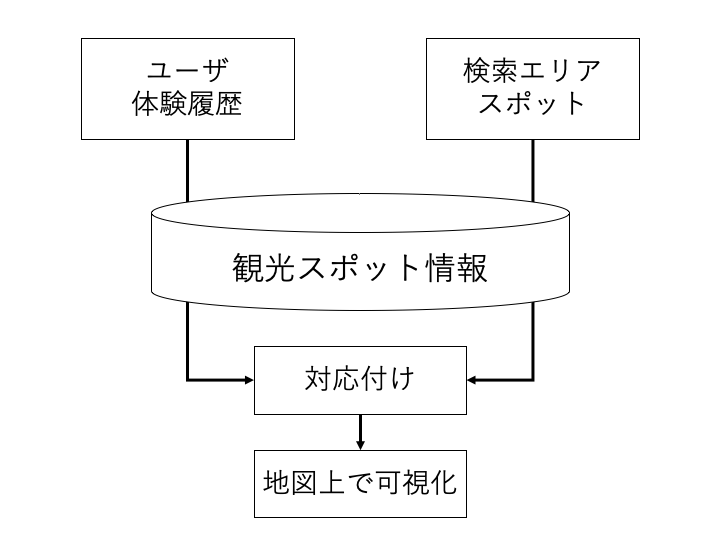
\includegraphics[width=0.9\textwidth]{figure/system_fig.png}
    \caption{観光支援システムの流れ}
    \label{fig:観光支援システムの流れ}
\end{figure}

まず,ユーザの体験履歴の中ていままで訪れたことがあるかつ気に入った観光スポットを入力する.
次に,これから行ってみたい都道府県やエリアを入力する.
そして,データベースで保存されている2016年10月までのじゃらんの観光スポットレビューデータを使って提案手法に適用することで,ユーザの未知な観光スポットに対する理解を支援するため,既に訪問したことがある観光スポットの特徴を用いて,未訪問エリアの観光スポットを説明するために対応付けを行う.

本研究における観光スポットの対応付けに関して,ユーザによって,その強調するべき特徴が変化する.
たとえば,日本の有名な観光スポットを履歴に持つユーザにとっての「東京都庁舍展望台」と「金閣寺」について考える.
このとき,「金閣寺」の相対的特徴は,お寺,金色,京都などである.
「東京都庁舍展望台」の相対的特徴は,展望,夜景,建物,新宿などが考えられる.

一方,京都の寺院を履歴に持つユーザにとっての「金閣寺」と「清水寺」について考える.
このとき,同じ「金閣寺」でもお寺や京都などは特徴にはならず,「金閣寺」の相対的特徴は,金色,金箔,輝きなどとなる.
「清水寺」の相対的特徴は,舞台や一望などである.

対応付けを行ったなあと,ユーザに未訪問スポットを説明するための観光スポット特徴語を抽出する.
最後に,地図上で既訪問スポットと未訪問スポットの対応関係と特徴語を可視化することで,ユーザが未訪問スポットに対する理解を容易化することを目指さす.

%%%%%%%%%%%%%%%%%%%
\section{関連研究}
%%%%%%%%%%%%%%%%%%%
% \subsection{類推思考に関する研究}
%%%%%%%%%%%%%%%%%%%
\subsection{体験履歴による検索や推薦システムに関する研究}
倉島ら\cite{Kurashima}は,Flickrに投稿された写真のジオタグ情報を人々の旅行履歴として利用した旅行ルート推薦手法を提案した.この手法では,ユーザの現在地から行きやすい場所とユーザの興味に合致した場所に移動しやすいと仮定し,行動モデルを生成している.
ユーザのジオタグ付き写真集合は,時間情報でソートすると個人の旅行履歴とみなすことができると考え,ジオタグ情報を利用してユーザの行動モデルを生成している.

Chengら\cite{Cheng}は,自由に利用できるコミュニティ投稿の写真を活用して,パーソナライズされた旅行のおすすめに焦点を当て,特定のユーザプロファイルまたは属性を考慮し,パーソナライズされた旅行の推奨を行うことを提案した.

観光地検索するとき,松本ら\cite{松本}はクチコミから特徴 語を抽出して利用する研究を行った.
抽出対象を任意の名詞として,4種類の手法,TFIDF,ATF(Average Term Frequency),ポアソン確率,エントロピーのうちどの手法が特徴語抽出に適しているのか検討を行った.
また,抽出した特徴語を利用した検索支援システムを試作し,実験を通して特徴語提示の効果を検証した.

嶋田ら\cite{嶋田}はWebから観光情報を抽出し,複数の特徴べクトルから観光地間の類似性を評価することで,観光地を推薦するシステムを提案した.
観光地の特徴べクトルは,知恵袋・ブログ上での共起キーワードと時系列分布,知恵袋上でのカテゴリ構造,観光地周辺施設,地図画像から生成した.
これらの特徴べクトルから観光地間の類似度の測定を行い,類似度の高い観光地を推薦した.

廣嶋ら\cite{廣嶋}は地理情報検索の際のクエリ入力支援として,提示する特徴語の抽出手法について研究を行った.
この手法では,各ブログ記事から特徴語候補の抽出および地点の特定を行った.
具体的には,特徴語の候補をWikipediaの見出し語に限定し,ポアソン確率を用いて特徴語抽出を行った.
また,地点の特定のための地名表現の抽出および緯度経度への変換の方法としては平野ら\cite{平野}の手法を用いた.

野守ら\cite{野守}は日本全国の観光地のクチコミデータを用いて,観光客が話題にする観光テーマを確率的に抽出し,そのテーマを軸として各観光地の特徴を定量的に評価した.
また,クチコミのテキストデータにテキストマイニングを実行して表現を抽出し,観光地ごとにその表現の出現頻度を集計したクロス集計表にPLSAを実行することで,観光客のクチコミだけに基づいた観光テーマの抽出と観光地の特徴分析を行なった.

このように多くの研究はユーザに合致する観光スポットの抽出や,一般的な特徴の抽出に焦点をあてているが,本研究では,ユーザの選択性を高めるために,個人化した特徴を抽出する点では異なる.

佐藤\cite{佐藤}はコスメアイテムに対してのクチコミからアイテムの特徴を抽出した.
また,それぞれのユーザのクチコミからアイテムに対する不満に相当する項目を抽出し,これらを基に各アイテムの特徴を可視化することで不満を解消するような新しい商品を提案した.

林ら\cite{林}は,レビュー中の評価表現とその評価対象に基づき,ユーザが書いた映画レビューから他者が書いた映画レビューを推薦する手法を提案した.
評価表現とその評価対象に基づく推薦を実現するために,レビュー中の「良い」や「良くない」などの肯定的または否定的な評価表現とその評価対象に着目した.

服部ら\cite{服部}はレビューを分析して,その価値観と繋がりの深い要素としてユーザの「こだわり」に着目し,その結果に基づくユーザモデリング手法について提案した.

従来のレビューを利用する手法では,クチコミを分析して,それぞれの嗜好や価値観を表す単語を重要視して,ユーザには単語レベルで提示されることが多い.
単語レベルの提示では,レビューの文章の雰囲気を損なうため,ユーザの入力としては,体験したことかつ気に入った観光スポットの全レビューを利用すると考えた.


%%%%%%%%%%%%%%%%%%%
%\subsection{地理的情報の可視化に関する研究}
\subsection{情報可視化に関する研究}
本研究では,地理的な情報の可視化と意味的な関係の可視化に取り込む.
地理的な情報の可視化としては,抽出した情報を地図上にマッピングするのが一般的であり,本研究もそれに従っている.
代表的な研究を以下に紹介する.
櫻川ら\cite{櫻川2015}は,ソーシャルメディア上にアップロードされた写真のジオタグ情報と撮影時刻に基づいて写真の撮影者を分類する手法を提案した.
分類された撮影者(観光者,在住者)ごとにホットスポットを可視化した.
また,ジオタグ情報と撮影時刻以外にテキストタグを加えて,写真が撮影された地域で行われるイベントの穴場スポットを発見し,地図上に提示する手法を提案した\cite{櫻川2016}.
倉田ら\cite{倉田2010}は,新しい観光情報サービスの形として「他の旅行者がどこで撮影したいか」というデータから観光ポテンシャルを可視化し,地図上に表示する方法を提案した.

%%%%%%%%%%%%%%%%%%%
%\subsection{意味的な関係性の可視化に関する研究}
意味的な関係性の可視化としては,グラフモデル上でオブジェクト間のつながりを関連度を表現することが多い.
代表的な研究を以下に紹介する.
Kitamuraら\cite{Kitamura}は,一般的な物体認識を用いて,過去の個人旅行写真から推定したユーザの旅行の嗜好に基づき観光地を推薦する方法を提案した.
物体認識システムを用いて,写真で撮った被写体情報のキーワードを取得し,グラフ視覚化技術によってキーワードの共起を表現した.
また,グラフの視覚化技術に基づいて旅行写真付きのグラフを視覚化するユーザインターフェイスを紹介した.
上村ら\cite{上村2019}は,ユーザが投稿したタグ付き画像を用いたファッションスタイルの関係性の可視化手法を提案した.
ファッションスタイルは類似するタグを空間座標に固定することによって関係を表している.

本研究では,観光スポット間の意味的な対応関係を可視化するために,未訪問スポットは地図上で実在する座標に固定され,配置の自由があるのは既訪問スポットのみという制約がある.

%%%%%%%%%%%%%%%%%%%%%%%%%%%%%%%%%%%%%%%%%%
\chapter{ユーザの既訪問スポットの位置付けに基づく未訪問スポットの説明手法}
%%%%%%%%%%%%%%%%%%%%%%%%%%%%%%%%%%%%%%%%%%
\section{概要}
\section{未訪問スポットの説明手法}
\section{キーワード抽出に関する評価}
\section{対応付けに関する評価}
\section{未訪問スポット説明の有効性評価}



%%%%%%%%%%%%%%%%%%%%%%%%%%%%%%%%%%%%%%%%%%
\chapter{地図上における未訪問スポットの説明性向上のための観光スポットの対応関係可視化手法}
%%%%%%%%%%%%%%%%%%%%%%%%%%%%%%%%%%%%%%%%%%
\section{概要}
\section{観光スポット間の対応関係を用いた可視化}
\section{対応関係の可視化評価}


%%%%%%%%%%%%%%%%%%%%%%%%%%%%%%%%%%%%%%%%%%
\chapter{考察}
%%%%%%%%%%%%%%%%%%%%%%%%%%%%%%%%%%%%%%%%%%


%%%%%%%%%%%%%%%%%%%%%%%%%%%%%%%%%%%%%%%%%%
\chapter{結論}
%%%%%%%%%%%%%%%%%%%%%%%%%%%%%%%%%%%%%%%%%%



%%%%%%%%%%%%%%%%%%%%%%%%%%%%%%%%%%%%%%%%%%
% 謝辞
\acknowledge{謝辞}
%%%%%%%%%%%%%%%%%%%%%%%%%%%%%%%%%%%%%%%%%%
修士課程での研究全般に渡ってご指導賜りました北山大輔准教授に厚く御礼申し上げます.

お忙しい中貴重な時間を割いて副指導教員およぶ副査を引き受けてくださり,ご指導賜りました三木良雄教授に感謝致します.

同様に,お忙しい中貴重な時間を割いて副査を引き受けてくださり,ご指導賜りました〇〇教授に感謝致します.

% また,学士学位論文に関するご指導も含め,3年間に渡ってご指導賜りました北山大輔准教授に感謝致します.
研究室配属からの3年間に渡って,切磋琢磨し心の支えにもなってくれた歴代のインタラクティブメディア研究室メンバ全員に感謝致します.

最後に,名前を書き切ることはできませんが,両親をはじめ,私のこれまでの人生を支えてくださった全ての方に心から感謝いたします.
ありがとうございました.


%%%%%%%%%%%%%%%%%%%%%%%%%%%%%%%%%%%%%%%%%%
% 参考文献
\references{参考文献}%タイトル変更可能
%%%%%%%%%%%%%%%%%%%%%%%%%%%%%%%%%%%%%%%%%%
\bibliographystyle{junsrt}
\bibliography{man}
%bibtexを使う方は,以下をコメントアウトし,上記を有効にする。スタイルは適宜変更のこと。
% \begin{thebibliography}{99}
%     \bibitem{c1} (雑誌の場合;雑誌とは論文誌等のこと)著者名, ``標題, '' 雑誌名, 巻, 号, pp.A--B, Month, 年.
%     \bibitem{c2} (著書,編書の場合)著者名, 書名, 編者名, 発行所, 発行都市名, 発行年.
%     \bibitem{c3} (著書の一部を引用する場合)著者名, ``標題, '' 書名, 編者名, 章番号またはpp.A--B, 発行所, 発行都市名, 発行年.
%     \bibitem{c4} (国際学会論文集の場合)著者名, ``標題, '' 会議名, no.A, pp.B--C, 都市名, 国名, Month, 年.
%     \bibitem{c5} (国内学会,研究会論文集の場合)著者名, ``標題, '' 学会論文集名, vol.A, no.B, pp.C--D, 都市名, 国名, Month, 年.
%     \bibitem{Kurashima}
%         T. {Kurashima}, T. {Iwata}, G. {Irie} and K. {Fujimura},
%         ``Travel Route Recommendation Using Geotags in Photo Sharing Sites,"
%         In Proceedings of the 19th ACM International Conference on Information and Knowledge Management,
%         pp.579-588, 2010
%     \bibitem{Kurashima}
%         R. {Kitamura} and T. {Itoh},
%         ``Tourist Spot Recommendation Applying Generic Object Recognition with Travel Photos,"
%         In 2018 22nd International Conference Information Visualisation (IV),
%         pp.1-5, 2018
%     \bibitem{Cheng}
%         A.J. {Cheng}, Y.Y. {Chen}, Y.T. {Huang} and W.H. {Hsu},
%         ``Personalized travel recommendation by mining people attributes from community-contributed photos,"
%         In Proceedings of the 19th ACM international conference on Multimedia,
%         pp.83-92, 2011
%     \bibitem{松本}
%         松本 敦志, 杉本 徹,
%         ``クチコミから抽出した特徴語を利用する観光地検索支援,"
%         第75回全国大会講演論文集,
%         vol.2013, no.1, pp.307-308, 2013
% \end{thebibliography}



%%%%%%%%%%%%%%%%%%%%%%%%%%%%%%%%%%%%%%%%%%%%%%%%%%%%%%
% 発表実績
\publications{本研究に関する発表}
%%%%%%%%%%%%%%%%%%%%%%%%%%%%%%%%%%%%%%%%%%%%%%%%%%%%%%
\begin{thepublication}
%
\publicationtype{論文}
\item \underline{潘健太}, 北山大輔, ``説明性向上のためのユーザレビューを用いた観光スポットの対応付け手法," 情報処理学会論文誌データベース, 第84号, 2019.
%
\publicationtype{査読付き会議}
\item \underline{Kenta Han}, Daisuke Kitayama, ``An Explanation Method of Unfamiliar Tourist Spots based on Roles of User's Familiar Spots," Lecture Notes in Engineering and Computer Science: Proceedings of The International MultiConference of Engineers and Computer Scientists 2019, Hong Kong, pp358-362, 13-15 March, 2019.
%
\publicationtype{研究会}
\item \underline{潘健太}, 北山大輔, ``ユーザの既訪問スポットの位置付けに基づく未訪問スポットの説明手法," 第11回データ工学と情報マネジメントに関するフォーラム(DEIM Forum 2019), H7-2, 2019
\item \underline{潘健太}, 北山大輔, ``地図上における未訪問スポットの説明性向上のための観光スポットの対応関係可視化手法," 観光情報学会第20回研究発表会, 2019
%
% \publicationtype{全国大会}
% \item \underline{1st Author}, 2nd Author, 3rd Author, Last Author, ``Title,'' Conference, Year.
%
\end{thepublication}


%%%%%%%%%%%%%%%%%%%%%%%%%%%%%%%%%%%%%%%%%%%%%%%%%%%%%%
% その他の発表実績
\publications{その他の発表実績}
%%%%%%%%%%%%%%%%%%%%%%%%%%%%%%%%%%%%%%%%%%%%%%%%%%%%%%
\begin{thepublication}
\publicationtype{研究会}
\item \underline{潘健太}, 北山大輔, ``ユーザのレビュー選択に基づく観光スポット検索手法," 第10回データ工学と情報マネジメントに関するフォーラム(DEIM Forum 2018), H1-2, 2018
\item \underline{潘健太}, 北山大輔, ``観光スポット検索のためのユーザのレビュー選択と特徴抽出に関する考察," 電子情報通信学会技術研究報告, vol. 118, no. 107, DE2018-5, pp. 21-24, 2018
\end{thepublication}


%%%%%%%%%%%%%%%%%%%%%%%%%%%%%%%%%%%%%%%%%%%%%%%%%%%%%%
% 受賞
\publications{受賞}
%%%%%%%%%%%%%%%%%%%%%%%%%%%%%%%%%%%%%%%%%%%%%%%%%%%%%%
\begin{thepublication}
\publicationtype{査読付き会議}
\item \underline{Kenta Han}, Daisuke Kitayama, ``An Explanation Method of Unfamiliar Tourist Spots based on Roles of User's Familiar Spots," Lecture Notes in Engineering and Computer Science: Proceedings of The International MultiConference of Engineers and Computer Scientists 2019, Hong Kong, pp358-362, 13-15 March, 2019.
\end{thepublication}


%%%%%%%%%%%%%%%%%%%%%%%%%%%%%%%%%%%%%%%%%%%%%%%%%%%%%%
% 研究室内部用の資料
\begin{domestic}
%%%%%%%%%%%%%%%%%%%%%%%%%%%%%%%%%%%%%%%%%%%%%%%%%%%%%%
\chapter{ファイルの場所}
本論文のファイル一式は研究室共有の...に保存してあります。実験プロジェクト等は研究室共有の...に保存してあります。


\chapter{引き継ぎ資料}
実験プロジェクトの使用法や,その他端書きは研究室共有の...に保存してあります。



%%%%%%%%%%%%%%%%%%%%%%%%%%%%%%%%%%%%%%%%%%
% 文書の終わり
%%%%%%%%%%%%%%%%%%%%%%%%%%%%%%%%%%%%%%%%%%
\end{domestic}
\eof%End-Of-File
%%%\end{document}は不要です
